\chapter{System Architecture and Workflow}
\label{chapter:system-architecture}
Humans are known for their ability to combine existing elements and create something new. We had a large number of frameworks and solutions to chose from and in the following sections we are going to talk about the various architecture and technology choices.
Also, we are going to present the workflow of the system.

\section{Recommendation System Architecture} 
\label{sec:architecture}

\begin{figure}[h]
\caption{System Architecture}
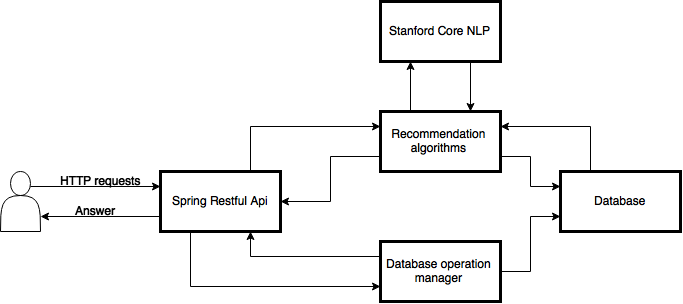
\includegraphics[width=1.0\textwidth]{src/img/architecture.png}
\end{figure}

As we can see in Figure 3.1, the user can interact with our system through a REST api which is provided by Spring Framework's MVC (Model-View-Controller). Based on the controller called by the user, the database operation manager, which uses the databse or the Recommendation algorithm is called, which uses the Stanford Core NLP framework and databse. We used a REST api since it is very easy to use and we needed a NLP framework in order to improve our recommendations. The database is needed for persistence between sessions, fast access to our items and storing our data on the disk, since it is impossible to keep it all in the RAM memory.

\subsection{Programming languages}
\label{sec:programming-languages}
There were a multitude of programming languages to chose from.
In the following subsections we are going to discuss what languages we chose, why and for what purpose.
We were influenced in our choices, by our previous technical experiences, by the ease of use of the presented technologies, the community support and documentation available.

\subsubsection{Java}
\label{sec:programming-languages-java}
Java\footnote{https://java.com} is a general purpose language that is class based, object oriented and concurrent. 
It is designed to have as few implemmentation dependencies as possible and be a "write once, run anywhere" type of language, meaning that compiled java code can run on all platforms that support java, without the need of recompilation.
Java applications are typically compiled to bytecode that can run on any Java virtual machine (JVM) regardless of the computer architecture.

It is a language that supports multiple paradigms, as:  object-oriented, structured, imperative, functional, generic, reflective, concurrent. In our implemmentation we used the imperative, object-oriented and concurrent paradigms. By combining the object-oriented and imperative paradigms we managed to obtain a well structured and easy to read code base. By using the concurrent paradigm we are taking full advantage of the current multi-core arhitectures.
Another reason for choosing Java is the great community and documentation. At the time of writing this document, Java was the most used language in the industry. Due to this, we can easily find support and documentation on any framework and problem we may stumble upon during the implemmentation of this system. Also, a great variety of frameworks exist for this language.

\subsubsection{Javascript}
\label{sec:programming-languages-javascript}
Javascript is a high level, dynamic, untyped and interpreted programming language. Alongside CSS and HTML, Javascript is one of the pillars of the current World Wide Web. In the last couple of years it has gained a great popularity in the detriment of action script, which was a programming language for the Adobe Flash Player. This movement towards Javascript is also because most mobile devices do not support Adobe Flash Player.
Even though, Javascript may also be used as a backend programming language, since the launch of Node.js, which is  an open source, cross-platform runtime environment for server-side and networking applications, the most common usage of Javascript is as a client side scripting language. This means that the Javascript code is sent along with the HTML to the browser, which then interprets it. A great advantage is the fact that the execution of the javascript code is done on the client, thus, in order to use it you just need to serve a file to the client.

In our implemmentation we used Javascript and Node.js to create a demo application which easily integrates with our Recommender System. Javascript was used to create the graphical user interface, since we have an abundance of frameworks that enable us to create a quick and beautiful user interface. Because of various security issues, Javascript is not allowed to make cross domain requests, so Node.js was used in order to create a proxy between our Recommender System and the Javascript client. Also, Node.js was used to serve the files to the client.
Also, in order to better show our Recommender System's capabilities, a Chrome plugin was built that could easily integrate with Adobe's existing platform.
Since, Javascript is one of the pillars of the World Wide Web and our Recommender System was meant to easily integrate with a web application, Javascript was the first choice for our demo applications.


\subsection{Frameworks}
\label{sec:frameworks}
A framework is like a black box that offers certain functionalities to it's user and does not require him to have any knowledge of what is going on behind the scenes
The basic principle of a framework is: Not having to reinvent the wheel. By using them we can build faster and better software.
Faster, because it allows the programmer to focus on implemmentation specific code, while re-using generic modules, without being tied to the framework itself.
Better, because a framework ensures you that the code you are running is in full compliance with the industry's rules. It is structured, and both upgradable and maintanable.
In the following sections we describe the frameworks used by our system and why we made those choices.

\subsubsection{Spring Framework}
\label{sec:frameworks-spring-framework}
Spring framework\footnote{http://projects.spring.io/spring-framework/} is one of the most popular Java application frameworks. It is an open source platform, which appeared in 2003 and it offers a wide range of modules, like testing, transaction management, Model-view-controller, remote access framework, etc. 
From all these modules, we use only the Model-view-controller part, in order to create the RESTful api of our system.
The only difference between a traditional MVC controller and a RESTful controller is the fact that in place of the server rendering the result on a view, it will just write an object's data, directly to a HTTP response, in a JSON format.
\lstset{caption=Spring framework REST controller code, label=lst:spring-framework-rest-controller}
\lstinputlisting{src/code/SpringController.java}
As we can see in the above \autoref{lst:spring-framework-rest-controller}, adding a controller is easy and we can set the request method and required parameters.
We can also return a model, in JSON format, if needed. The only requirement is that the object returned has getters for each of it's attributes.
Due to easiness of use, great popularity and the fact that it enforces some of the java principles, by requiring us to set accessors to the used classes, we can say that Spring is the best choice for our system. 

\subsubsection{Apache HBase}
\label{sec:frameworks-hbase}
Hbase\footnote{http://hbase.apache.org/} is an open source, non relational and distributed databse, modeled after Google's Big Table. It is written in Java, which is a great advantage, since it is really easy to integrate with our existing code.
Unlike realational databases, the structure of a non relational database is very simillar to that of a hash map. This grants us an easier control over the content of the database and faster access time. Most of the operations can be done in constant time. HBase also has an api that supports multiple types of queries, simillar in functionality to those of a SQL database.
Since HBase is a distributed database, it also obeys the CAP theorem, also known as Brewer's theorem, which states that it is impossible for a distributed system to provide all of the following:

\begin{itemize}
	\item Consistency - The same data is seen by all nodes at the same time.
	\item Availability - If a number of nodes from your cluster fail, then the system will still be available.
	\item Partition tolerance - The system will continue to operate, even if the cluster has been split into multiple partitions, that are unable to exchange messages, due to network failures.
\end{itemize}

Hbase has appeared due to the need of processing massive amounts of data for the purpose of language processing and is a CP type system. 
Since, we needed a fast and reliable database, that could process the large amounts of text data that we obtained from our articles and which could easily be integrated with Java, HBase was the right choice for our recommender system. Another reason for choosing HBase was the fact that it has a great community and support. 

\subsubsection{Stanford CoreNLP}
\label{sec:frameworks-stanford-corenlp}
Stanford CoreNLP\cite{manning-EtAl:2014:P14-5} provides us with a set of NLP processing tools. Even though, this is a powerful tool, capable to give the base forms of words, their parts of speech, whether they are names of companies, people, etc., normalize dates, times, and numeric quantities, and mark up the structure of sentences in terms of phrases and word dependencies, indicate which noun phrases refer to the same entities, indicate sentiment, etc we use only a small part of it's capabilities.
Stanford CoreNLP is an integrated framework which can be used with ease and we can choose what tools to enable or disable by simply setting the options given to the framework. 
From all the existing options we use only the "tokenize", "ssplit", "pos" and "lemma", which we describe below.

The purpose of the "tokenize" option is to tokenize the text. We need this in order to split large chunks of text into separate words, thus being able to lemmatize each word and use it to get better similarity between articles.
The purpose of the "ssplit" property is that of splitting the text into sentences for the future analysis of the meaning of each word based on the context of the sentence in order to reduce it to a basic form by using the lemma property.
The purpose of the "pos" option is to enable the Part-Of-Speech Tagger (POS Tagger) of the Stanford CoreNLP. 
A POS Tagger is a tool that reads text in a language and assigns parts of speech to each word, such as noun, verb, adjective, etc..
We need it in order to determine what part of speach each word is and based on that, we can reduce the word to a simpler form, by using the "lemma" property.
The purpose of the "lemma" property is that of applying the lemmatization process to all the tokens of the document.
Lemmatization is the process of grouping different forms of a word so they can be processed as a single item.
In most of the languages, words are used in several inflicted forms. For example the verb "to be" may appear as "was", "am", "being", etc. The base form of the word, in this case, would be the one you can find in the dictionary, "be" and this is called the lemma of the word. If we combine the part of speech, determined from the context,  with the base form of the word, we get something called the lexeme of the word. 

Another process, closely related to lemmatisation is called stemming. The main difference is that in the stemming process we do not take into account the context of a word, but only the word itself, and therefore we ca not make a difference between words, based on the part of speech. For example, the word "beings", will always be reduced by a stemmer to the base form "be", which is wrong, if used as a noun "All beings are like each other in existing". The lemmatisation process will determine, based on the context, that the word is a noun and has the basic form "being". A stemmer will be able to reduce the word "walking" to the correct form "walk", just like a lemmatizer.

If the application does not need great accuracy, then a stemmer is recommended, since the running time is much faster and the implemmentation is simpler.
We chose a lemmatizer in order to increase the quality of our similarity results. The lemmatizer is used only in the article adding stage, when creating the TFIDF entries, in order to be able to make fast recommendations. If we need to compute word similarity, during the recommendation stage, then we are using the Levenshtein Distance or a simple word similarity algorithm, based on pairs of letters of the word, as presented in the Recommendation Algorithms chapter.

\lstset{caption=Stanford Core NLP lemmatizer code, label=lst:stanford-core-nlp}
\lstinputlisting{src/code/StanfordCoreNLP.java}

\subsubsection{Apache Maven}
\label{sec:frameworks-apache-maven}
Apache maven\footnote{https://maven.apache.org/} is a buid and project management system used primarily with Java. It's main functionalities are that of building a project and defining it's dependencies. A XML files is used to define the project's dependencies, repos from where they can be downloaded, the order in which the build executes and the required directors and plugins.
In order to be able to easily setup our system on different platforms, we needed a dependency system. Since Apache Maven is a popular system, compatible with Java, that has quite a long history and a great community it was our choice.

\section{Recommendation System Workflow} 
\label{sec:workflow}
There are multiple actions that you can request from the recommendation system through the Spring RESTful api.
In the following sections we describe the implemented use cases.
All the data is returned as a JSON object.

\begin{figure}
\caption{System Workflow}
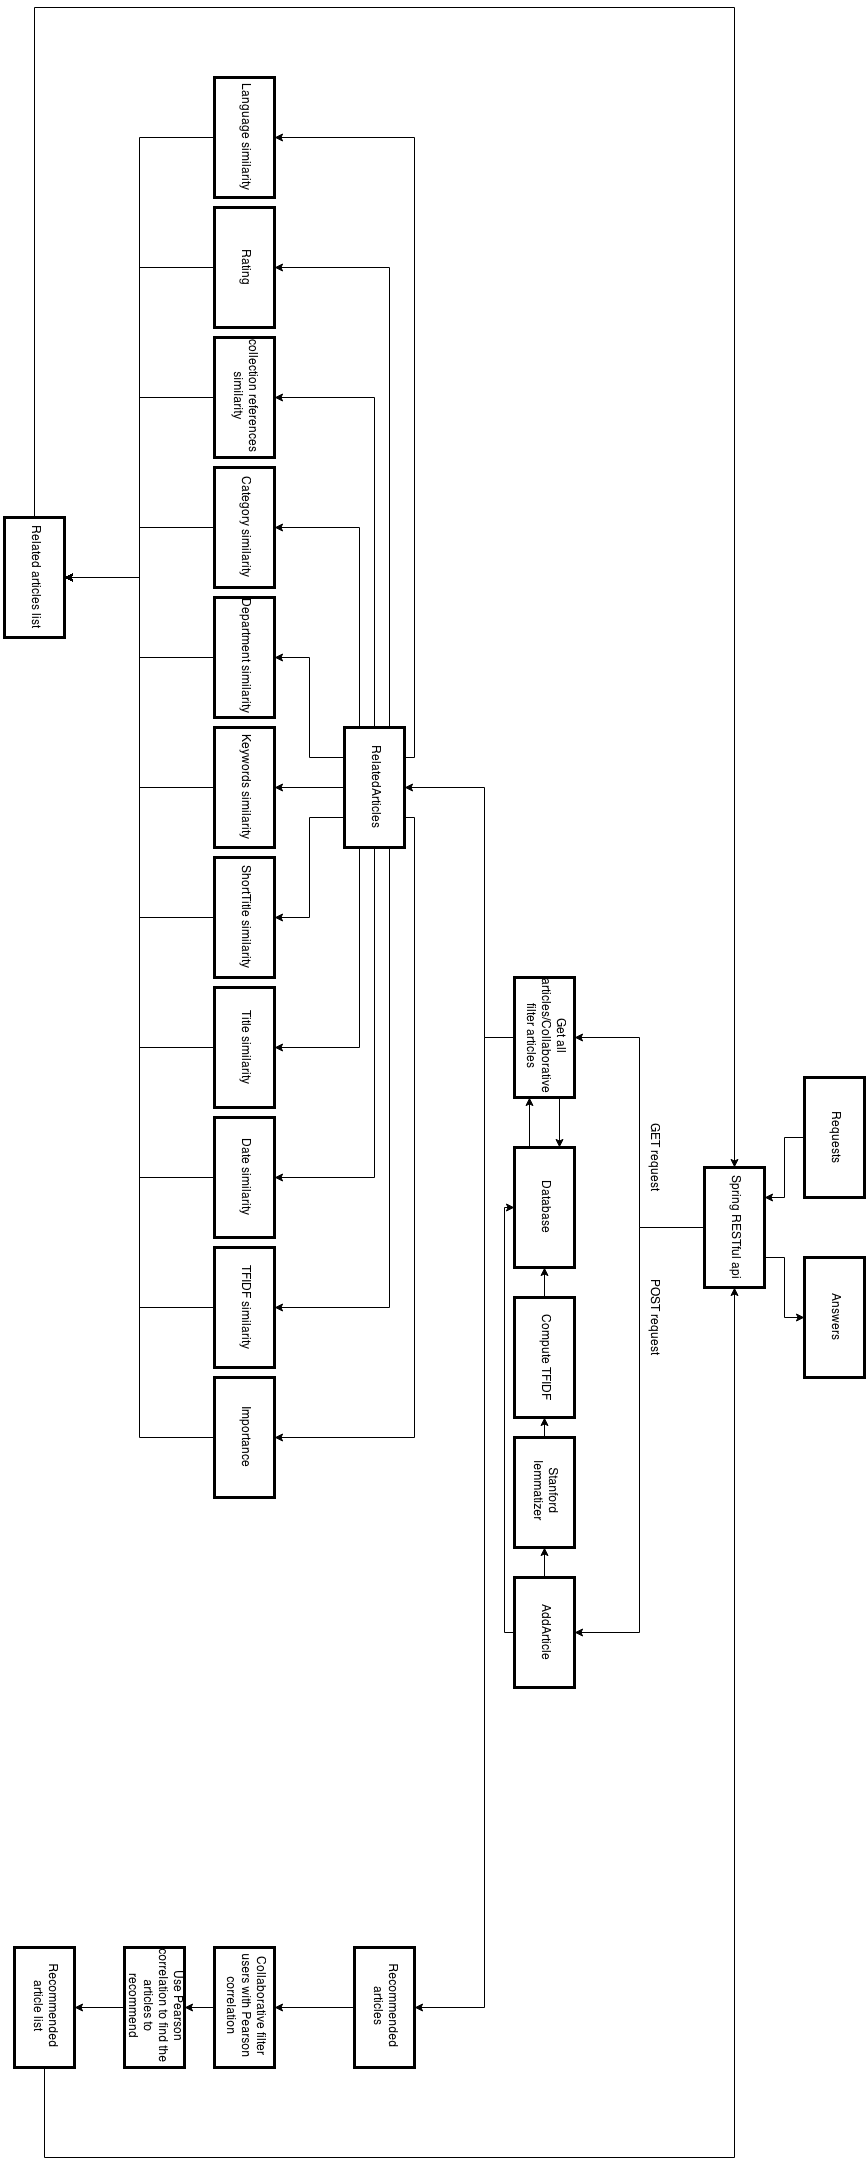
\includegraphics[width=\textwidth,height=\textheight,keepaspectratio]{src/img/workflow.png}
\end{figure}

\subsection{Add user}
\label{sec:workflow-add-user}
A PUT request is made to the RESTful api with the required data for adding a friend of an user.
The minimum data required for a user is the user id and friend id.
The request is intercepted by the api and the new friend is added to the user’s top friends list. If the operation is successful then the user receives “true”, otherwise the user is informed of the error. 

\subsection{Add user friend}
\label{sec:workflow-add-user-friend}
A PUT request is made to the RESTful api with the required data for adding a friend of an user.
The minimum data required for a user is the user id and friend id.
The request is intercepted by the api and the new friend is added to the user’s top friends list. If the operation is successful then the user receives “true”, otherwise the user is informed of the error. 

\subsection{Add user direct recommendation}
\label{sec:workflow-add-user-direct-recommendation}
A PUT request is made to the RESTful api with the required data for adding a direct user recommendation.
These are supposed to be recommendations made manually by a user.
The minimum data required is the user id and an item id.
The request is intercepted by the api and the user entry is fetched from the database and the new item is added to the items directly recommended list of the user. If the operation is successful then the user receives “true”,otherwise the user is informed of the error. 

\subsection{Delete user}
\label{sec:workflow-delete-user}
A DELETE request is made to the RESTful api with the required data for deleting an user.
The minimum required data is the user id
The request is intercepted by the api and the database entry is deleted. If the operation is successful then the user receives “true”, otherwise the user is informed of the error. 

\subsection{Update user article history}
\label{sec:workflow-update-user-article-history}
A PUT request is made to the RESTful api with the required data for updating an user article history
The read article history can be updated and a rating of a certain article can be added. 
The minimum required fields are the article id and the user id.
The request is intercepted by the api and the user entry is fetched from the database. The new item is added to the article history list of the user. If the operation is successful then the api returns “true”, otherwise the user is informed of the error. 

\subsection{Article recommendations based on friends direct recommendations}
\label{sec:workflow-friends-direct-recommendations}
A GET request is made to the RESTful api with the user id.
The request is intercepted by the api and all the directly recommended articles of the top friends of the user are returned.
The top friends list can be added manually through the api.
If a top friends list does not exist, one will be generated by using the user’s previous article history.
If the operation is successful then the user receives “true”, otherwise the user is informed of the error. 

\subsection{Add article}
\label{sec:workflow-add-article}
A PUT request is made to the RESTful api with the required data for adding a new article.
The request is intercepted by the api and the new article is added to the database.
The minimum required data is the article id.
If the operation is successful then the user receives “true”, otherwise the user is informed of the error.


\subsection{Get articles}
\label{sec:workflow-get-all-articles}
A GET request is made to the RESTful api in order to get the articles from the databse.
The user may specify how many articles he wishes to receive or hey may request for a specific article.
The articles are fetched from the database and returned to the user.
If the operation is successful then the user receives the article list, otherwise the user is informed of the error

\subsection{Get recommended articles}
\label{sec:workflow-get-recommended-articles}
A GET request is made to the RESTful api in order to get the recommended articles for a user
The minimum required data is the user id for whom we need the recommendation.
The system tries to guess how the user will rate the articles in the database, based on his previous ratings and the ratings of the other users he has the most common interests.
If the operation is successful then the user receives the top rated articles, otherwise the user is informed of the error.

\subsection{Get related articles}
\label{sec:workflow-get-related-articles}
A GET request is made to the RESTful api in order to get the related articles for an article.
The minimum required data is the article id for which we need the related articles. The user can also specify a max number of articles to be returned
The system intercepts the request and uses all the similarity methods from the presented workflow to calculate the similarity between every article in the database and the current article.
Each article has a value from 0 to 1 meaning the similarity with the article for which we requested the related articles.
The top related list is returned is if the operation is successful, otherwise the user is be informed of the error.


\subsection{Get articles related to a collection}
\label{sec:workflow-get-articles-related-to-collection}
A GET request is made to the RESTful api in order to get the related articles for  a collection.
The minimum required data is the collection article list.
By using the previous presented process of getting an article’s similarity score to another article, we get the similarity score of all the articles to all the collection articles. We sum up this scores and return the articles with the top similarity score, if the operation is successful, otherwise the user is informed of the error.

\subsection{Integration with chrome plugin}
\label{sec:workflow-integration-with-chrome-plugin}
If the articles in the current publication do not exist in the database, then the chrome extension adds them by doing specific requests to the application's api.
Once all the articles have been added, the user may start a view in which he can see the related articles.